
\resetcounters


\markboth{Yang and Szalay}{GPU-Based Visualization}


\title{A \ssindex{computing!GPU}GPU-Based \ssindex{visualization}Visualization Method for Computing \ssindex{astronomy!darm matter}Dark Matter Annihilation Signal}
\author{Lin~Yang and Alex~Szalay
\affil{Department of Physics \& Astronomy, Johns Hopkins University}}

\aindex{Yang, L.}
\aindex{Szalay, A.}

\begin{abstract}
We present a novel \ssindex{computing!GPU}GPU-based \ssindex{visualization}visualization method for computing the \ssindex{astronomy!darm matter}dark matter annihilation signal for cosmological \ssindex{astronomy!darm matter}dark matter \ssindex{astronomy!simulation}simulations. The technique increased the speed of rendering by more than 1,000 times. In a previous study, using a code running on regular CPUs, each particle's contribution was explicitly calculated pixel by pixel over a \ssindex{libraries!HEALPix}HEALPIX map, then remapped onto a \ssindex{astronomy!projections!Molleweide}Molleweide projection. Using Via Lactea II \ssindex{astronomy!simulation}simulation ($\sim$ 400M particles), it takes over 7 hours for a single thread CPU ($\sim$3 GHz) to complete an all-sky map with  NSIDE=512 resolution. Our novel method is based on a separate \ssindex{astronomy!projections!stereographic (STR)}stereographic projection for each hemisphere, and a hardware accelerated rendering \ssindex{data!pipelines!reduction}pipeline on a \ssindex{computing!GPU}GPU (\ssindex{libraries!OpenGL}\ssindex{software!tools!OpenGL}OpenGL). We project the particles instead of the celestial sphere to the tangent plane with a skewed flux profile appropriate for the\ssindex{astronomy!projections!stereographic (STR)} STR projection. \ssindex{libraries!OpenGL}\ssindex{software!tools!OpenGL}OpenGL's Point Sprite feature and shader language allow us to render those eccentric circular flux profiles at the rate of more than 10M particles per second. The new method can process a single snapshot of the Via Lactea II data in less than 1 minute with a single \ssindex{NVIDIA}NVIDIA GTX 480 \ssindex{computing!GPU}GPU, including I/O, with effective rendering time less than 24 seconds. Using an approximate normalization for the flux, accurate to 2.5\% in total flux, the rendering can be done in less than 13 seconds. The \ssindex{astronomy!projections!stereographic (STR)}stereographic images corresponding to the two hemispheres are then warped to an all-sky image in the \ssindex{astronomy!projections!Molleweide}Molleweide projection, and are in good agreement with the result from the regular CPU code, at similar resolution.

\end{abstract}

\section*{Introduction}
In a previous study \citet{Kuhlen:2008kr}, the whole sky map of \ssindex{astronomy!darm matter}dark matter annihilation \ssindex{astronomy!gamma-ray}Gamma-Ray signal is estimated from the VIALACTEA II (VL-II) \ssindex{astronomy!simulation}simulation to simulate Fermi-LAT's observation. The snapshot used is a 40 Mpc box with about 400 million particles. With a SPH kernel smoothing and certain approximation, each particle's cross section independent flux distribution is
\begin{equation}\label{fluxeq}
	F_i(\theta,\phi)\mathrm{d}\Omega = 
	\left\{\begin{aligned}
		N\frac{m_i\rho_i}{4\pi d_i^2} \exp\left(-\frac{3}2\frac{\delta\theta^2}{r_\theta^2}\right)\mathrm{d}\Omega  &\  & \delta\theta \le r_\theta \\
		0	&\   & \delta\theta > r_\theta\
	\end{aligned}\right. ,
\end{equation}
where $\delta\theta$ is the angular distance from $(\theta, \phi)$ to the particle's angular position; $r_\theta$ is the angular radius of the particle; and $\rho_i, m_i, d_i$ are the density, mass and distance of the i-th particle. With the help of \ssindex{libraries!HEALPix}HEALPIX \citep{Gorski:2005ku}, each particle's contribution is calculated and weight distributed in a certain pixel disk, as described by Equation~(\ref{fluxeq}). Calculating the pixel disc is an extremely inefficient process. Even though it's easy to parallelize and to run each particle in a single \ssindex{computing!GPU}GPU thread, the direct \ssindex{computing!architecture!CUDA}CUDA version of the CPU code is even slower. The reason is that the pixel distribution of each particle is highly varied (each particle has an average of 68 pixels on its HEALPIX disk, but with a standard deviation of 115, and there are more than 20k particles having more than 10k pixels). Sorting the particles based on the angular radius could largely reduce the threads skew, however the optimal \ssindex{computing!architecture!CUDA}CUDA code needs 1 hr more to run (GPU: GTX 480), compare to the \ssindex{computer languages!C++}C++ code, which requires about 7 hrs (~3 GHz CPU). 

In this paper, we propose a new method which could largely increase the speed. Due to the high inefficiency of querying HEALPIX pixel disks, we used \ssindex{astronomy!projections!stereographic (STR)}stereographic projection (STR) instead. In \S 1, we introduce the method we used; \S 2 shows the comparison between the new result and old result; \S 3 introduces some potential usage of the new method.


\section{\ssindex{computing!GPU}GPU Based\ssindex{astronomy!projections!stereographic (STR)} STR Projection (GSP) Method}
STR projection projects a circle on the sphere to a circle on the projection plane, whereas the center is projected to an off-center point. Hence the Gaussian profile of a particle's flux has been projected to a stretched Gaussian (see Fig~\ref{figstr}). 

\begin{figure}[htb]
\begin{center}
 \includegraphics[width=120mm]{part3/Yang_P045/P045_f1}
\caption{STR Projection. Circle on the sphere is projected to a circle on the projection plane.\label{figstr}}
\end{center}
\end{figure}

With STR, we use \ssindex{libraries!OpenGL}\ssindex{software!tools!OpenGL}OpenGL's Point Sprite feature to render the stretched Gaussians to squared billboards and add them together on the projection plane.\ssindex{astronomy!projections!stereographic (STR)} STR projection has a singular point at the north pole. In order to reduce distortion around the pole, we divided the  sphere into 2 hemispheres. The south hemisphere uses the north pole as the projection point and vise versa. The result is shown on (Fig~\ref{figsky}).

\begin{figure}[htb]
\begin{center}
 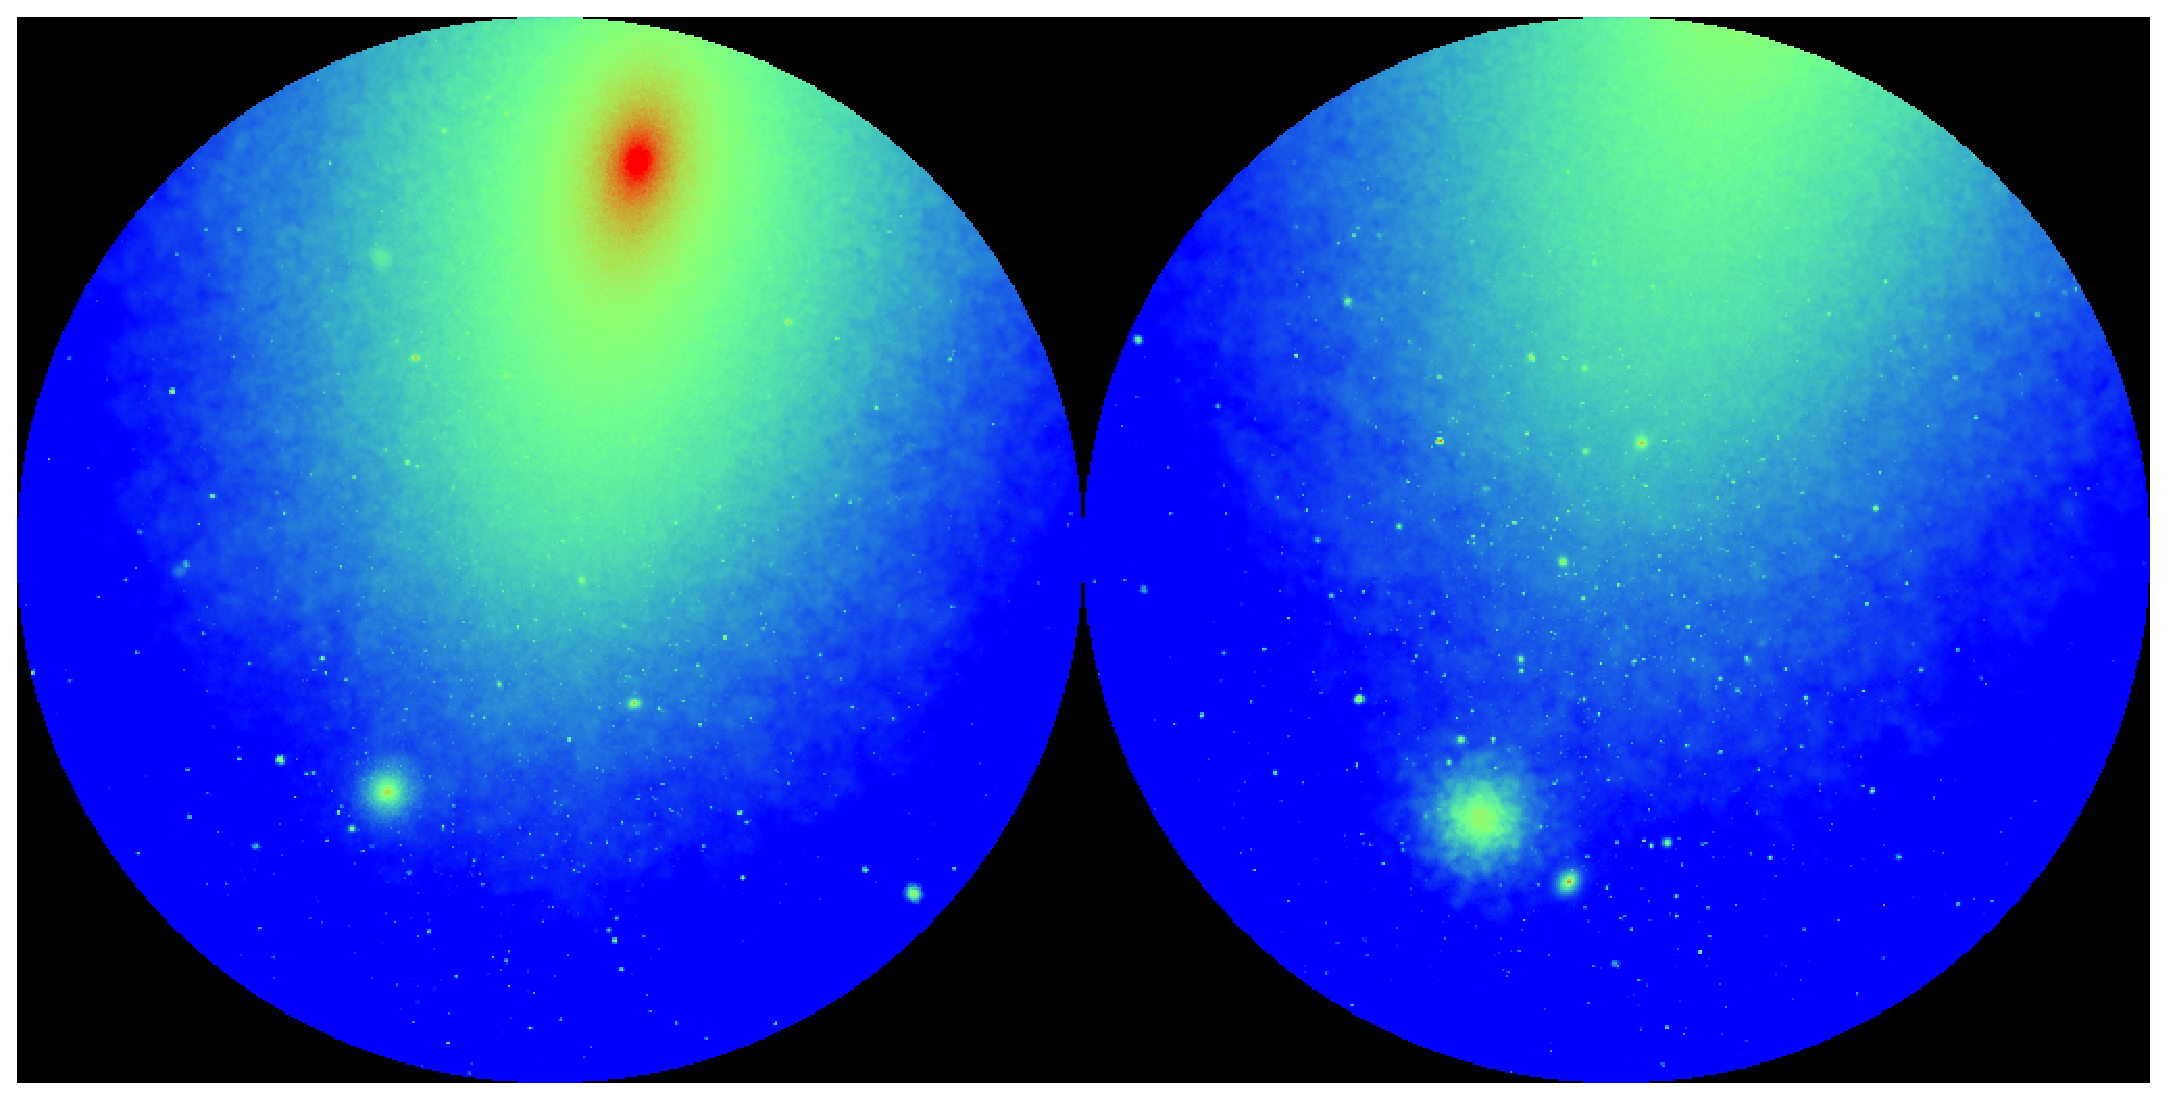
\includegraphics[width=80mm]{part3/Yang_P045/P045_f2}
\caption{ Point Sprite Rendering of Annihilation Signal. Every particle's Gaussian profile is projected to a stretched Gaussian. The sphere is divided into 2 hemispheres to reduce the distortion. Left is the north hemisphere, right is the south hemisphere. Color: Blue: -.5 ---- Red: 4.5;  Units: Log10[GeV$^2$ cm$^{-6}$ kpc].\label{figsky}}
\end{center}
\end{figure}

\section{Comparasion}
Both projection and \ssindex{computing!GPU}GPU rendering could add additional errors. In order to verify the result, we converted our result back to the \ssindex{libraries!HEALPix}HEALPIX map. As shown in (Fig~\ref{figcmp}), panel (a) shows the map of the original method, panel (b) shows the result of the GSP method. Their difference is shown in panel (c). The bright peaks appear in identical positions as the original method. Some errors is shown on very bright peaks, it may due to the float point error of \ssindex{computing!GPU}GPUs. The largest error is shown on the joint of the North and South sphere. We argue that, with good awareness of these, the physics is not changed and hence the error is negligible. 

\begin{figure}[htb]
\begin{center}
 \includegraphics[width=140mm]{part3/Yang_P045/P045_f3}
\caption{Mollweide Projection of the All Sky Flux Maps. (a) is generated by the original slow method; (b) is generated by the GSP method. (c) shows their difference. \label{figcmp}}
\end{center}
\end{figure}

The original \ssindex{libraries!HEALPix}HEALPIX (\ssindex{computer languages!C++}c++/\ssindex{packages!IDL}idl version) method (with NSIDE = 512), which runs for nearly 7 hrs to complete the computation on an Intel(R) Xeon(R) CPU X7350 2.93GHz CPU. For revised \ssindex{computing!architecture!CUDA}CUDA code, running on a \ssindex{NVIDIA}NVIDIA GTX 480 GPU, it still takes 1 hr. However, with our method, running on the same \ssindex{computing!GPU}GPU, the time consumed is only about 24 seconds (with resolution $512\times512\times2$ pixels). Using an analytical normalization method, the time consuming could be reduced to $~12$ seconds. Moreover, increasing resolution only turns out to have a linear increase in the consumed time, e.g., with resolution $1024\times1024\times2$ pixels, the time cost for the analytical method is about 20 seconds (all the above measurements do not contain the I/O time). 

\begin{figure}[htb]
\begin{center}
 \includegraphics[width=110mm]{part3/Yang_P045/P045_f4}
\caption{Fig~4: GSP Method Works as \ssindex{Virtual Observatory (VO)}Virtual Observatory. Left panel simulates observing at the Galaxy center on earth with a view angle of 78 degree (each pixel is about 9 arcmin, similar to Fermi-LAT’s observation). Right panel is the radial profile of the signal distribution, restoring \citet{Kuhlen:2008kr}'s Fig~4.  \label{figapp}}
\end{center}
\end{figure}

\section{Potential Application}
Our method is universal to any \ssindex{astronomy!darm matter}dark matter \ssindex{astronomy!simulation}simulation, it could tremendously increase the analysis speed when a \ssindex{astronomy!simulation}simulation is computed. In addition to generating an all-sky map, it could also work as a \ssindex{Virtual Observatory (VO)}virtual observatory. As shown on Fig~\ref{figapp} (left panel), by specifying a view angle, and only project a single sphere, we simulate a \ssindex{astronomy!gamma-ray}Gamma-Ray observation (without convolving with a\ssindex{astronomy!point spread function (PSF)} PSF). The resolution used here is about $9$ arcmin/pixel, similar to Fermi-LAT's angular resolution. Fig~\ref{figapp} (right panel) is angular distribution of the \ssindex{astronomy!gamma-ray}Gamma-ray, restoring \citet{Kuhlen:2008kr}'s Fig~4. 

\section{Conclusion}
STR projection works very well to visualize the \ssindex{astronomy!darm matter}dark matter annihilation signal. With small error caused by the \ssindex{computing!GPU}GPU rendering and re-projection, the speedup GSP gains is remarkable. Compared to the previous code, GSP is about 1000 times faster. Our method could be used as a preview of any \ssindex{astronomy!darm matter}Dark Matter \ssindex{astronomy!simulation}simulation before being formally analyzed. If high precision is required, we still recommend the previous \ssindex{libraries!HEALPix}HEALPIX method. However, in a speed/time preferred situation, our method is definitely a good choice. 

\acknowledgements LY would like to thank Tam$\mathrm{\acute{a}}$s Budav$\mathrm{\acute{a}}$ri for suggestions, discussions, and help. LY would like to thank Tam$\mathrm{\acute{a}}$s Szalay, Kai Buerger and several other people for the help on \ssindex{computing!GPU}GPU programming. LY would like to thank Mattias Lee for the help with the operating system and discussions. 

\bibliographystyle{asp2010}
\bibliography{editor}
